\documentclass[aspectratio=169]{beamer}

\usetheme{Madrid}
\usecolortheme{default}
\setbeamertemplate{navigation symbols}{}

\usepackage[T5,T1]{fontenc}
\usepackage[utf8]{inputenc}
\usepackage[english,vietnamese]{babel}
\usepackage{graphicx}
\usepackage{booktabs}
\usepackage{tikz}
\usetikzlibrary{arrows.meta,positioning}

\definecolor{accent}{RGB}{14,88,109}
\definecolor{soft}{RGB}{236,244,247}
\setbeamercolor{title}{fg=accent}
\setbeamercolor{frametitle}{fg=accent}
\setbeamercolor{structure}{fg=accent}
\setbeamercolor{block title}{fg=white,bg=accent}
\setbeamercolor{block body}{bg=soft}
\graphicspath{{assets/figures/}}
\newcommand{\figsource}[1]{{\raggedright\tiny Source: #1\par}}

\title[Sparse View 3D Reconstruction]{Sparse\_View\_3D\_Reconstruction}
\subtitle{Project Proposal Slides}
\author[CV Team]{Nguyễn Ngọc Minh, Kiều Sơn Tùng, Đặng Thịnh Tường Minh}
\institute[CV 2025.2]{Computer Vision 2025.2}
\date{\today}

\begin{document}

\begin{frame}
  \titlepage
\end{frame}

\begin{frame}{Team Setup}
  \begin{block}{Student information}
    \begin{itemize}
      \item Nguyễn Ngọc Minh -- 20235533
      \item Kiều Sơn Tùng -- 20235571
      \item Đặng Thịnh Tường Minh -- 20235528
    \end{itemize}
  \end{block}

  \vspace{0.4cm}
  \begin{block}{Presentation goal}
    Present the final RGB-D/source-depth reconstruction setting and the Run 30
    source-ray correction result after the RGB-only learned extensions failed
    reconstruction-level gates.
  \end{block}
\end{frame}

\begin{frame}{Motivation}
  \begin{itemize}
    \item 3D reconstruction is important because 3D representations help
    machines understand spatial structure, depth, and object relationships more
    accurately.
    \item Practical 3D capture often has only a small number of usable images.
    \item Classical high-quality pipelines depend on accurate camera poses or
    expensive scene-specific optimization.
    \item Sparse views increase ambiguity because cross-view correspondence is
    harder to establish reliably.
    \item A fast, generalizable method for unseen scenes would be useful for
    robotics, AR/VR, navigation, and scalable environment digitization.
  \end{itemize}
\end{frame}

\begin{frame}{Problem Statement}
  \begin{block}{Core question}
    How can we reconstruct unseen scenes accurately and efficiently when only
    2 to 5 input views are available?
  \end{block}

  \vspace{0.3cm}
  \begin{columns}[T]
    \column{0.48\textwidth}
    \textbf{Key constraints}
    \begin{itemize}
      \item Unseen scene at test time
      \item Sparse overlapping images
      \item No per-scene optimization
    \end{itemize}

    \column{0.48\textwidth}
    \textbf{Expected outcome}
    \begin{itemize}
      \item Robust geometry recovery
      \item Stable performance under view reduction
      \item Practical runtime per scene
    \end{itemize}
  \end{columns}
\end{frame}

\begin{frame}{Objectives}
  \begin{enumerate}
    \item Build a strong sparse-view MV-DUSt3R+ baseline for 2--5 views.
    \item Diagnose why RGB-only learned reliability, match filtering, and
    monodepth correction fail reconstruction-level gates.
    \item Switch the final setting to posed RGB-D views with known camera
    intrinsics/extrinsics.
    \item Validate Run 30 source-depth correction on overall, occlusion, and
    repeated/wrong-depth ambiguity subsets.
  \end{enumerate}
\end{frame}

\begin{frame}{Final Hypothesis}
  \begin{block}{Working hypothesis}
    Candidate deletion is too risky for sparse-view reconstruction. When input
    source depth is available, anchoring source rays to metric RGB-D geometry
    should correct wrong-depth candidates while preserving recall.
  \end{block}

  \vspace{0.3cm}
  \begin{itemize}
    \item Keep the useful MV-DUSt3R+ candidate set instead of over-filtering it
    \item Use source depth, poses, and intrinsics to correct 3D locations
    \item Test the result on occlusion and repeated/wrong-depth hard subsets
  \end{itemize}
\end{frame}

\begin{frame}{Proposed Contributions}
  \begin{alertblock}{Our contribution}
    Beyond benchmarking DUSt3R and MV-DUSt3R+, we first identify which
    sparse-view components help, then propose a supervised extension for
    the failure cases that heuristic filters could not solve.
  \end{alertblock}

  \vspace{0.12cm}
  \begin{itemize}
    \item \textbf{View selection for far-reference issue:} replace random sparse-view
    sampling with policies that balance scene coverage, viewpoint diversity,
    and overlap.
    \item \textbf{Honest ablation of heuristic fusion/filtering:} test confidence,
    multi-view support, occlusion, and ambiguity signals separately.
    \item \textbf{Supervised reliability extension:} replace failed hand-written
    filters with learned occlusion reliability and repeated-structure match
    disambiguation heads.
  \end{itemize}
\end{frame}

\begin{frame}{Contribution Details}
  \footnotesize
  \begin{block}{1. View selection for far-reference issue}
    \begin{itemize}
      \item Compare \textbf{random baseline}, \textbf{coverage-aware},
      \textbf{diversity-aware}, and \textbf{hybrid} sparse-view policies.
      \item The goal is to reduce far-reference failures while preserving
      co-visibility under 2--5 input views.
    \end{itemize}
  \end{block}

  \begin{block}{2. Heuristic ablation before adding learned modules}
    \begin{itemize}
      \item Evaluate \(C\), \(S_{mv}\), \(M\), occlusion penalties, and
      ambiguity penalties independently.
      \item If a module reduces F-score or completeness, keep it out of the
      final pipeline and report the failure explicitly.
    \end{itemize}
  \end{block}

  \begin{block}{3. Supervised occlusion and ambiguity heads}
    \begin{itemize}
      \item Train an \textbf{Occlusion-Aware Reliability Head} to keep
      occluded-but-valid points and reject floating/wrong geometry.
      \item Train a \textbf{Repeated-Structure Disambiguation Head} using
      reciprocal matches, descriptor margin, reprojection, and cycle error.
    \end{itemize}
  \end{block}
\end{frame}

\begin{frame}{Learned Extension After Ablation}
  \footnotesize
  \begin{block}{Why not keep tuning heuristic filters?}
    Early ablations show that hand-written occlusion and ambiguity filters can
    remove valid geometry and reduce completeness. The next step is supervised
    reliability learning rather than stronger manual penalties.
  \end{block}

  \begin{itemize}
    \item \textbf{OARH:} predict whether each candidate point should be kept,
    using confidence, visibility, occlusion, reprojection, depth disagreement,
    and multi-view agreement features.
    \item \textbf{RSDH:} predict whether repeated-structure matches are valid,
    using MASt3R reciprocal matching, feature margin, 3D disagreement, and
    cycle consistency.
    \item \textbf{Fine-tuning policy:} freeze MV-DUSt3R+ first; only later
    unfreeze the confidence head and last decoder blocks if validation improves.
  \end{itemize}
\end{frame}

\begin{frame}{Proposed Method}
  \begin{columns}[T]
    \column{0.34\textwidth}
    \begin{itemize}
      \item Primary method: \textbf{MV-DUSt3R+}
      \item Single-stage feed-forward multi-view reconstruction
      \item Final setting uses sparse posed RGB-D views
      \item Run 30 adds source-depth correction after MV-DUSt3R+
      \item Our study focuses on robustness, hard cases, and runtime
    \end{itemize}

    \vspace{0.15cm}
    \figsource{Tang et al., MV-DUSt3R+, project page and paper}

    \column{0.66\textwidth}
    \centering
    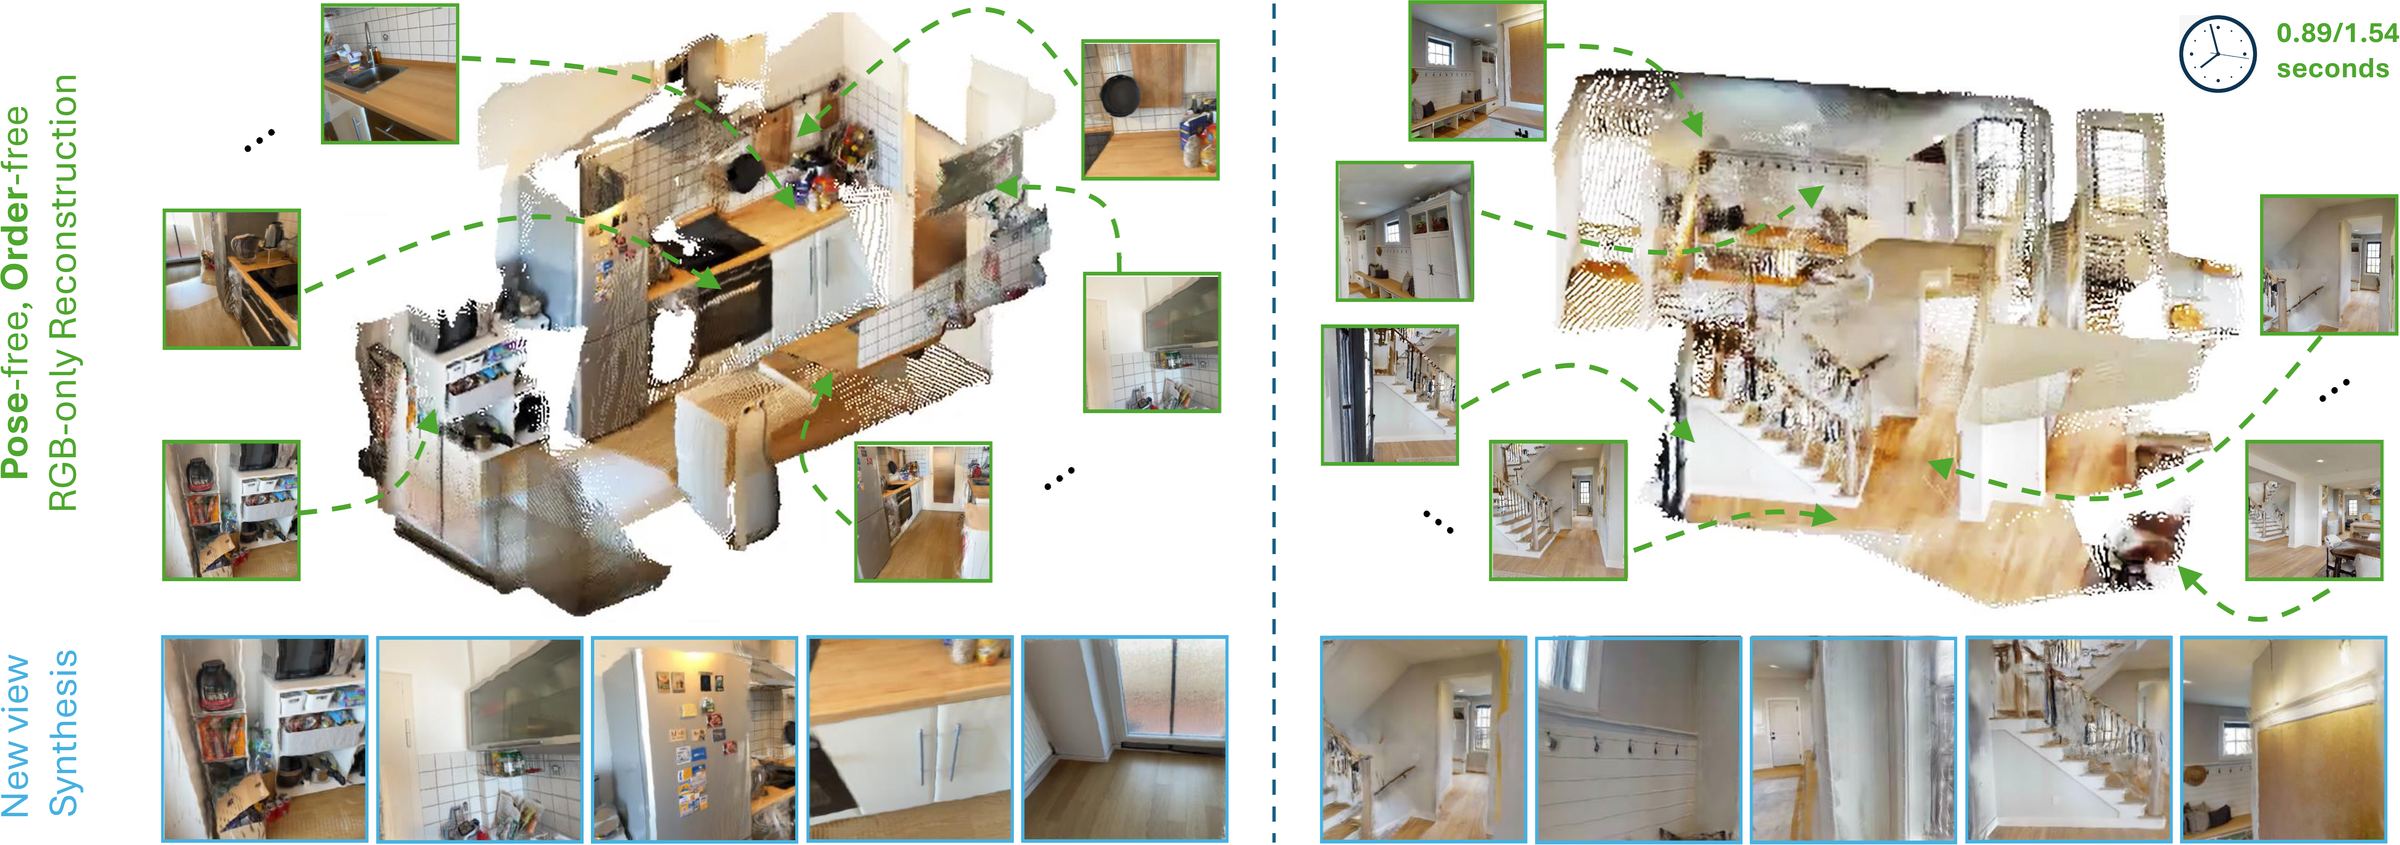
\includegraphics[width=\linewidth]{mv_overview_slide.png}
  \end{columns}
\end{frame}

\begin{frame}{Architecture Comparison}
  \begin{columns}[T]
    \column{0.49\textwidth}
    \centering
    \textbf{DUSt3R baseline}\par
    \vspace{0.1cm}
    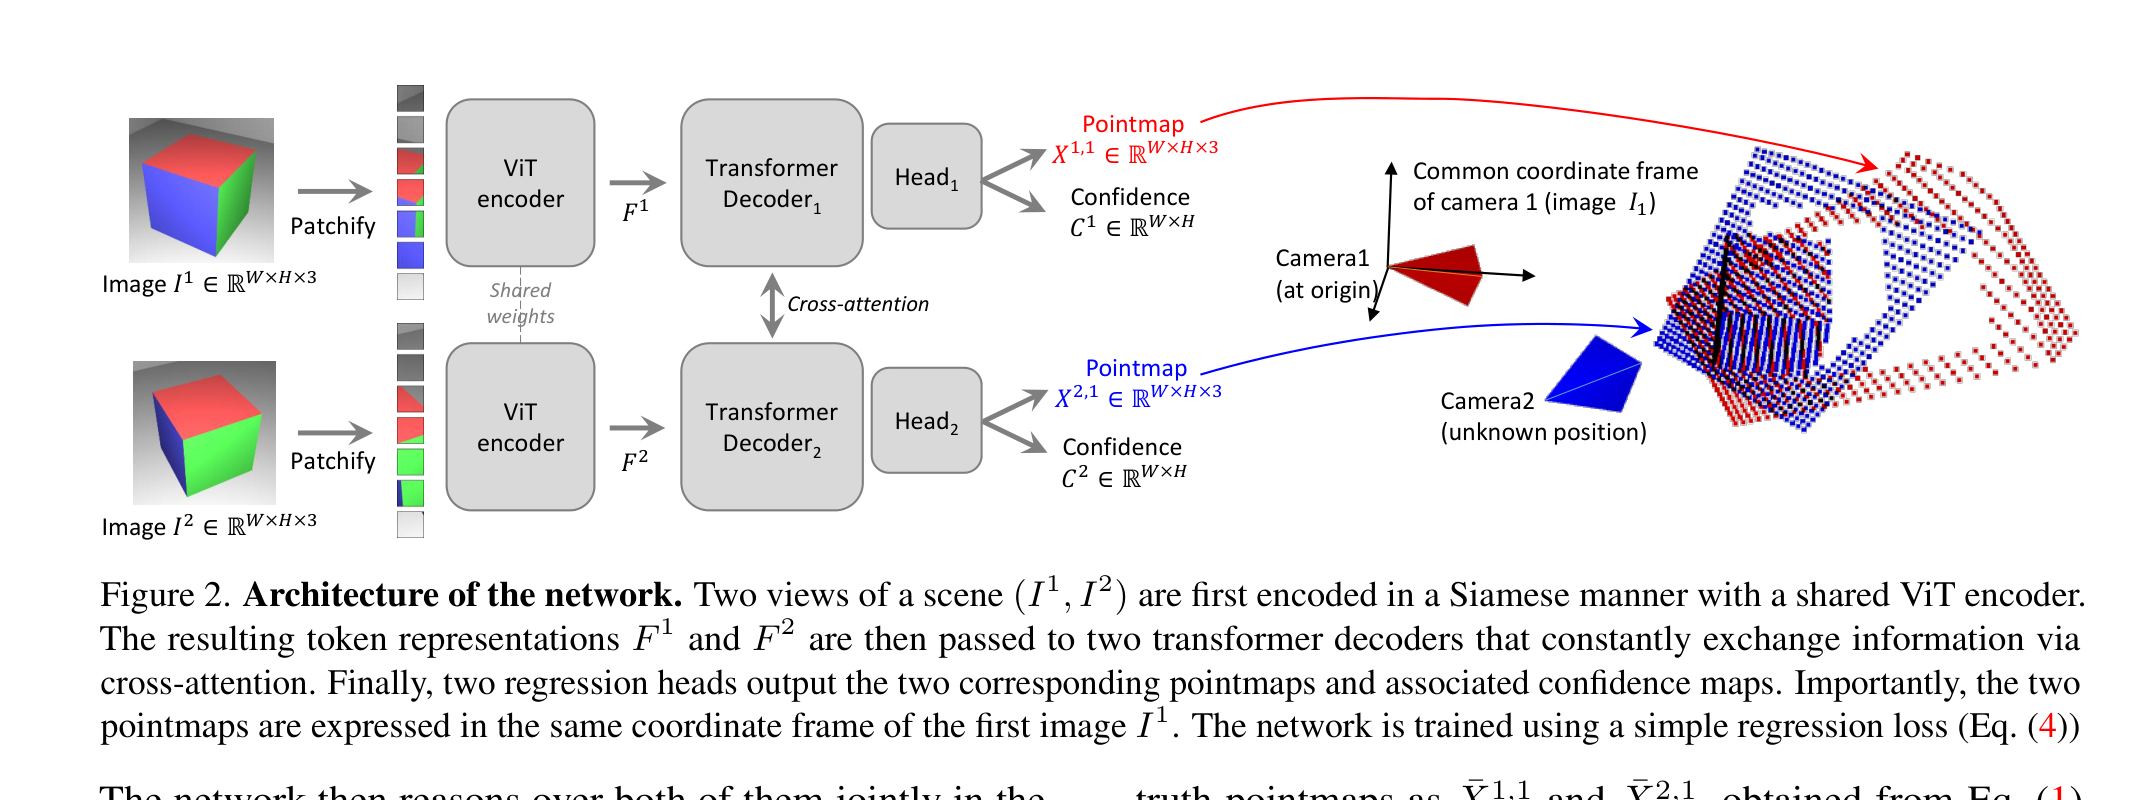
\includegraphics[width=\linewidth]{dust3r_arch_crop.png}

    \vspace{0.08cm}
    {\scriptsize Pairwise reasoning with cross-attention between two views}

    \column{0.49\textwidth}
    \centering
    \textbf{MV-DUSt3R+ main method}\par
    \vspace{0.1cm}
    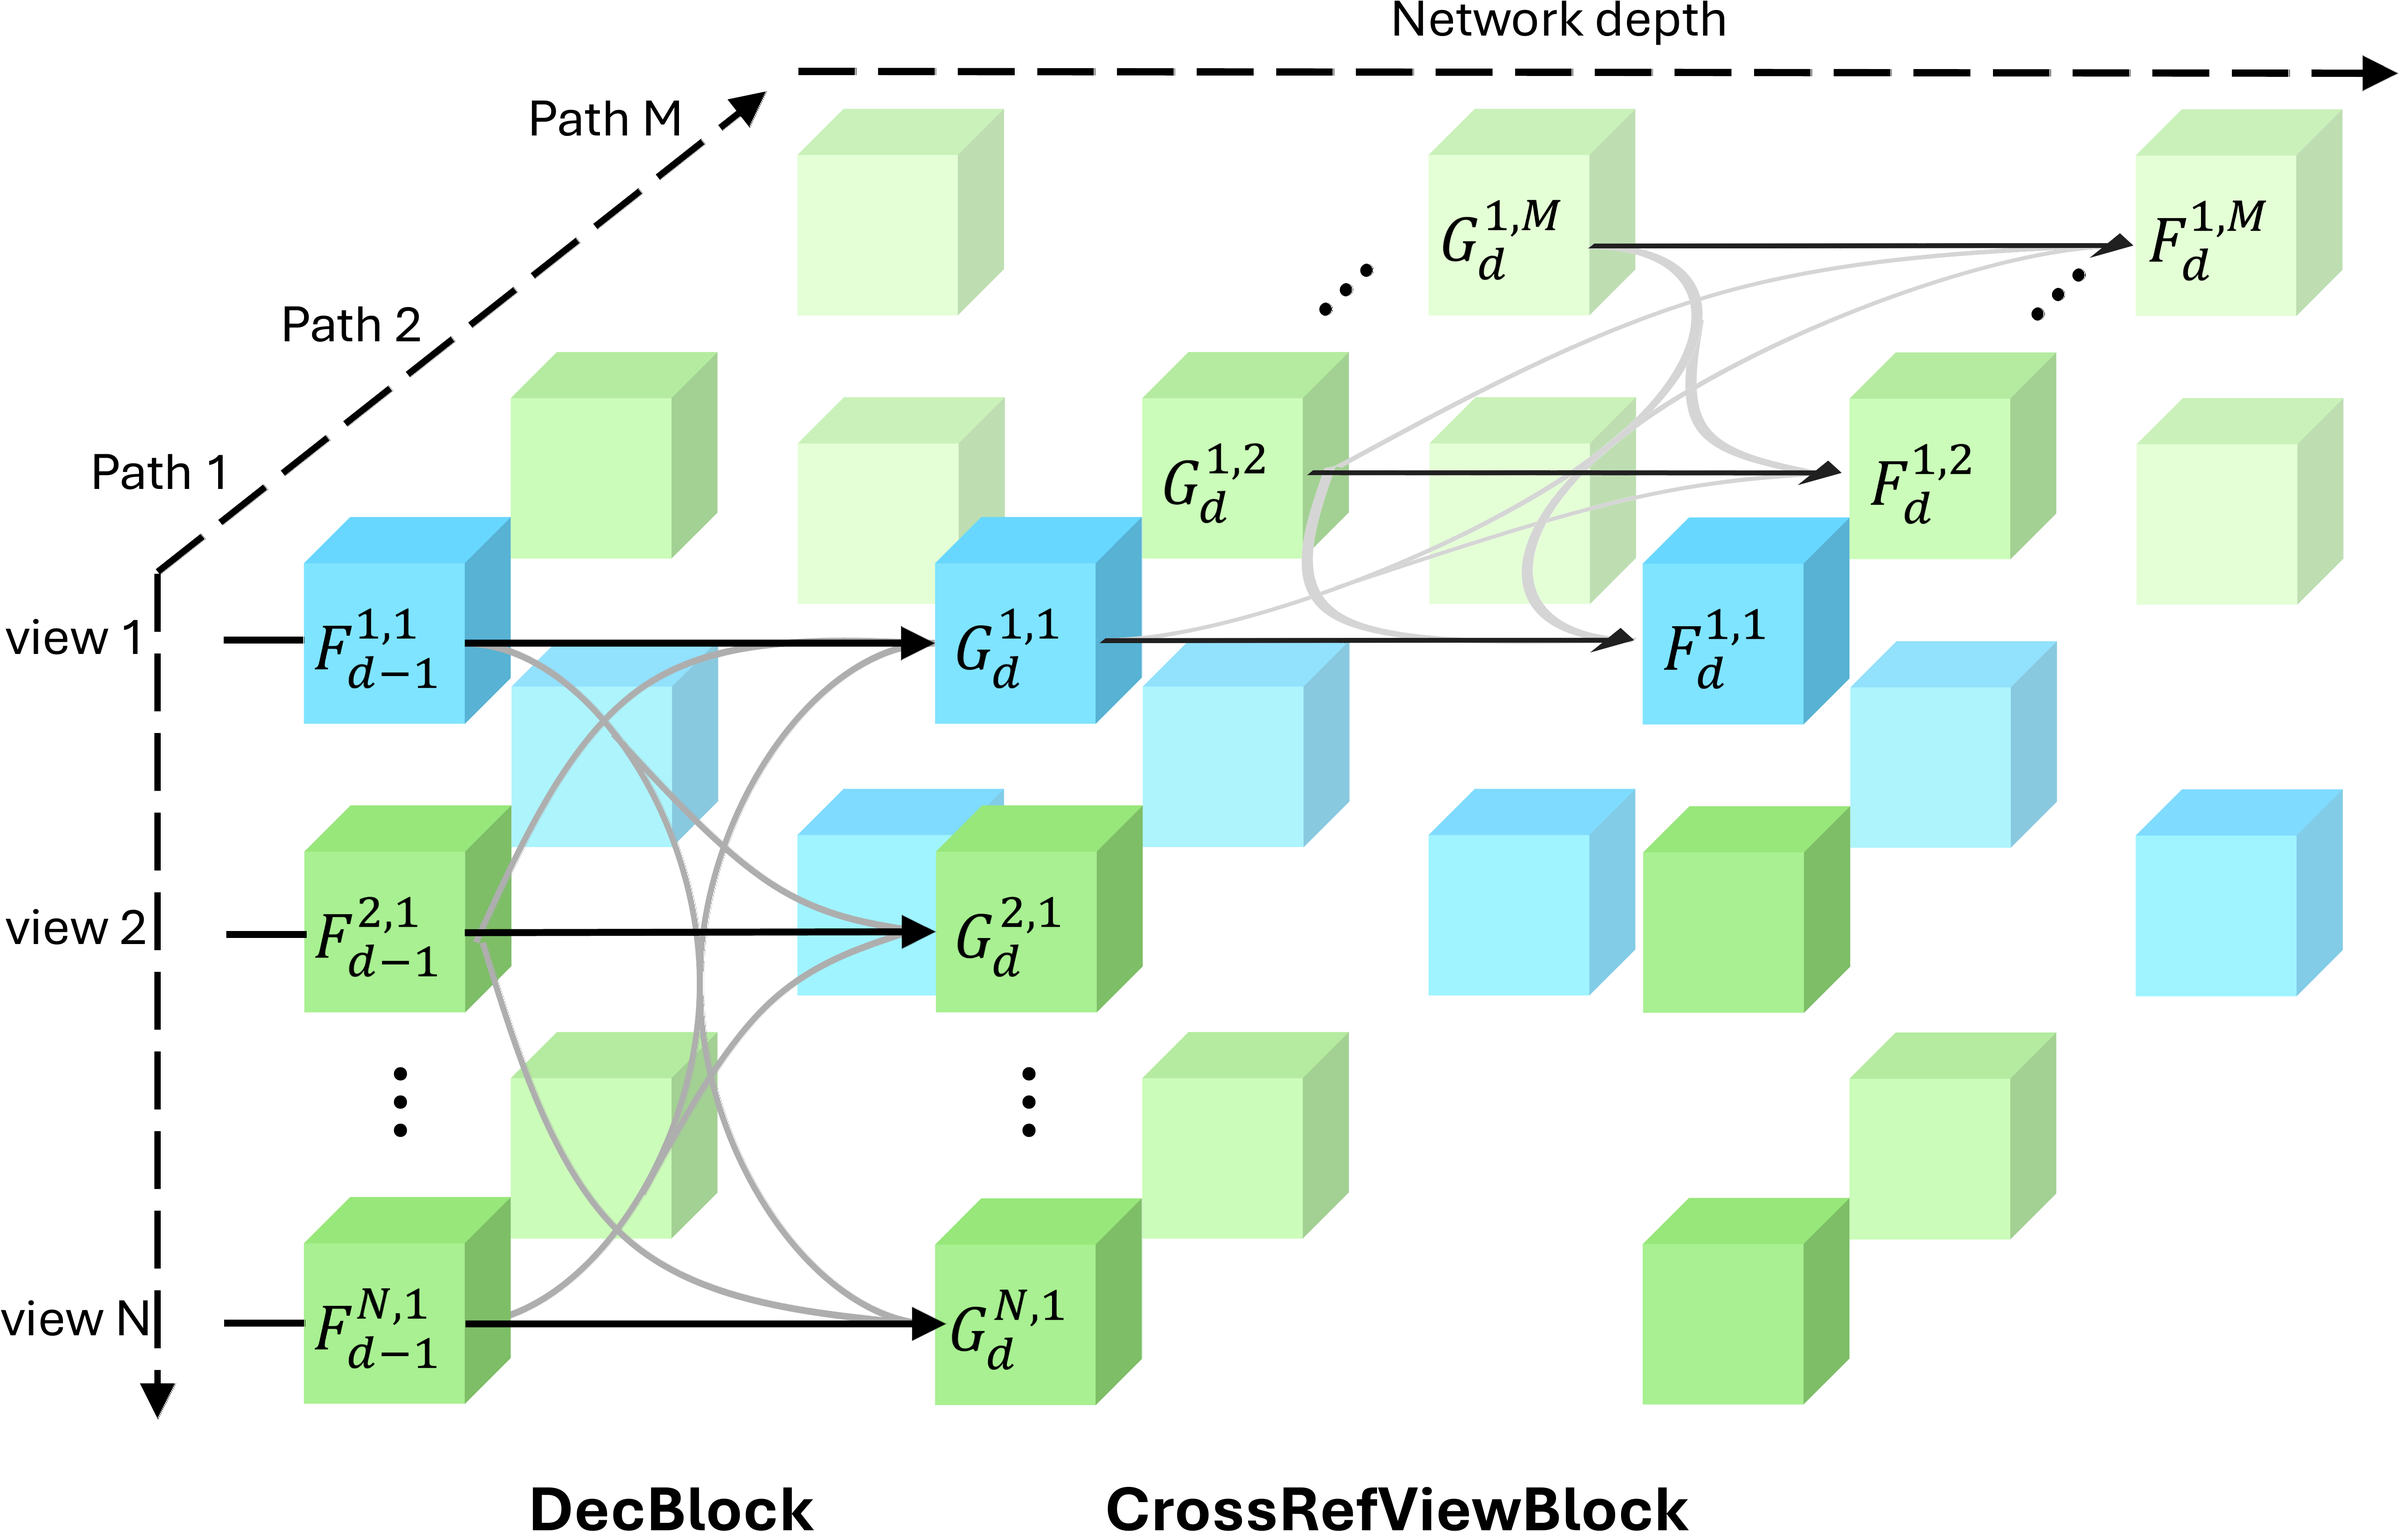
\includegraphics[width=\linewidth]{mv_arch_slide.png}

    \vspace{0.08cm}
    {\scriptsize Multi-path design with cross-reference-view information flow}
  \end{columns}

  \vspace{0.12cm}
  \figsource{Left: Wang et al., DUSt3R, CVPR 2024. Right: Tang et al., MV-DUSt3R+, project page/paper}
\end{frame}

\begin{frame}{Why MV-DUSt3R+ vs DUSt3R?}
  \small
  \begin{tabular}{p{0.22\textwidth} p{0.33\textwidth} p{0.33\textwidth}}
    \toprule
    \textbf{Aspect} & \textbf{DUSt3R} & \textbf{MV-DUSt3R+} \\
    \midrule
    Processing style & Pairwise reconstruction & Joint multi-view reconstruction \\
    Global consistency & Requires later alignment & Built into one forward pass \\
    Sparse-view behavior & Can accumulate pairwise errors & More robust cue fusion \\
    Runtime trend & Slower as views increase & Better scaling with more views \\
    Role in project & Reference baseline & Main candidate method \\
    \bottomrule
  \end{tabular}

  \vspace{0.22cm}
  \begin{itemize}
    \item DUSt3R is still a strong baseline, so the comparison is direct and meaningful.
    \item MV-DUSt3R+ is the candidate generator for both the Run 30 RGB-D
    reference and the target estimated-depth correction step.
  \end{itemize}
\end{frame}

\begin{frame}{Quantitative Evidence from the Paper}
  \centering
  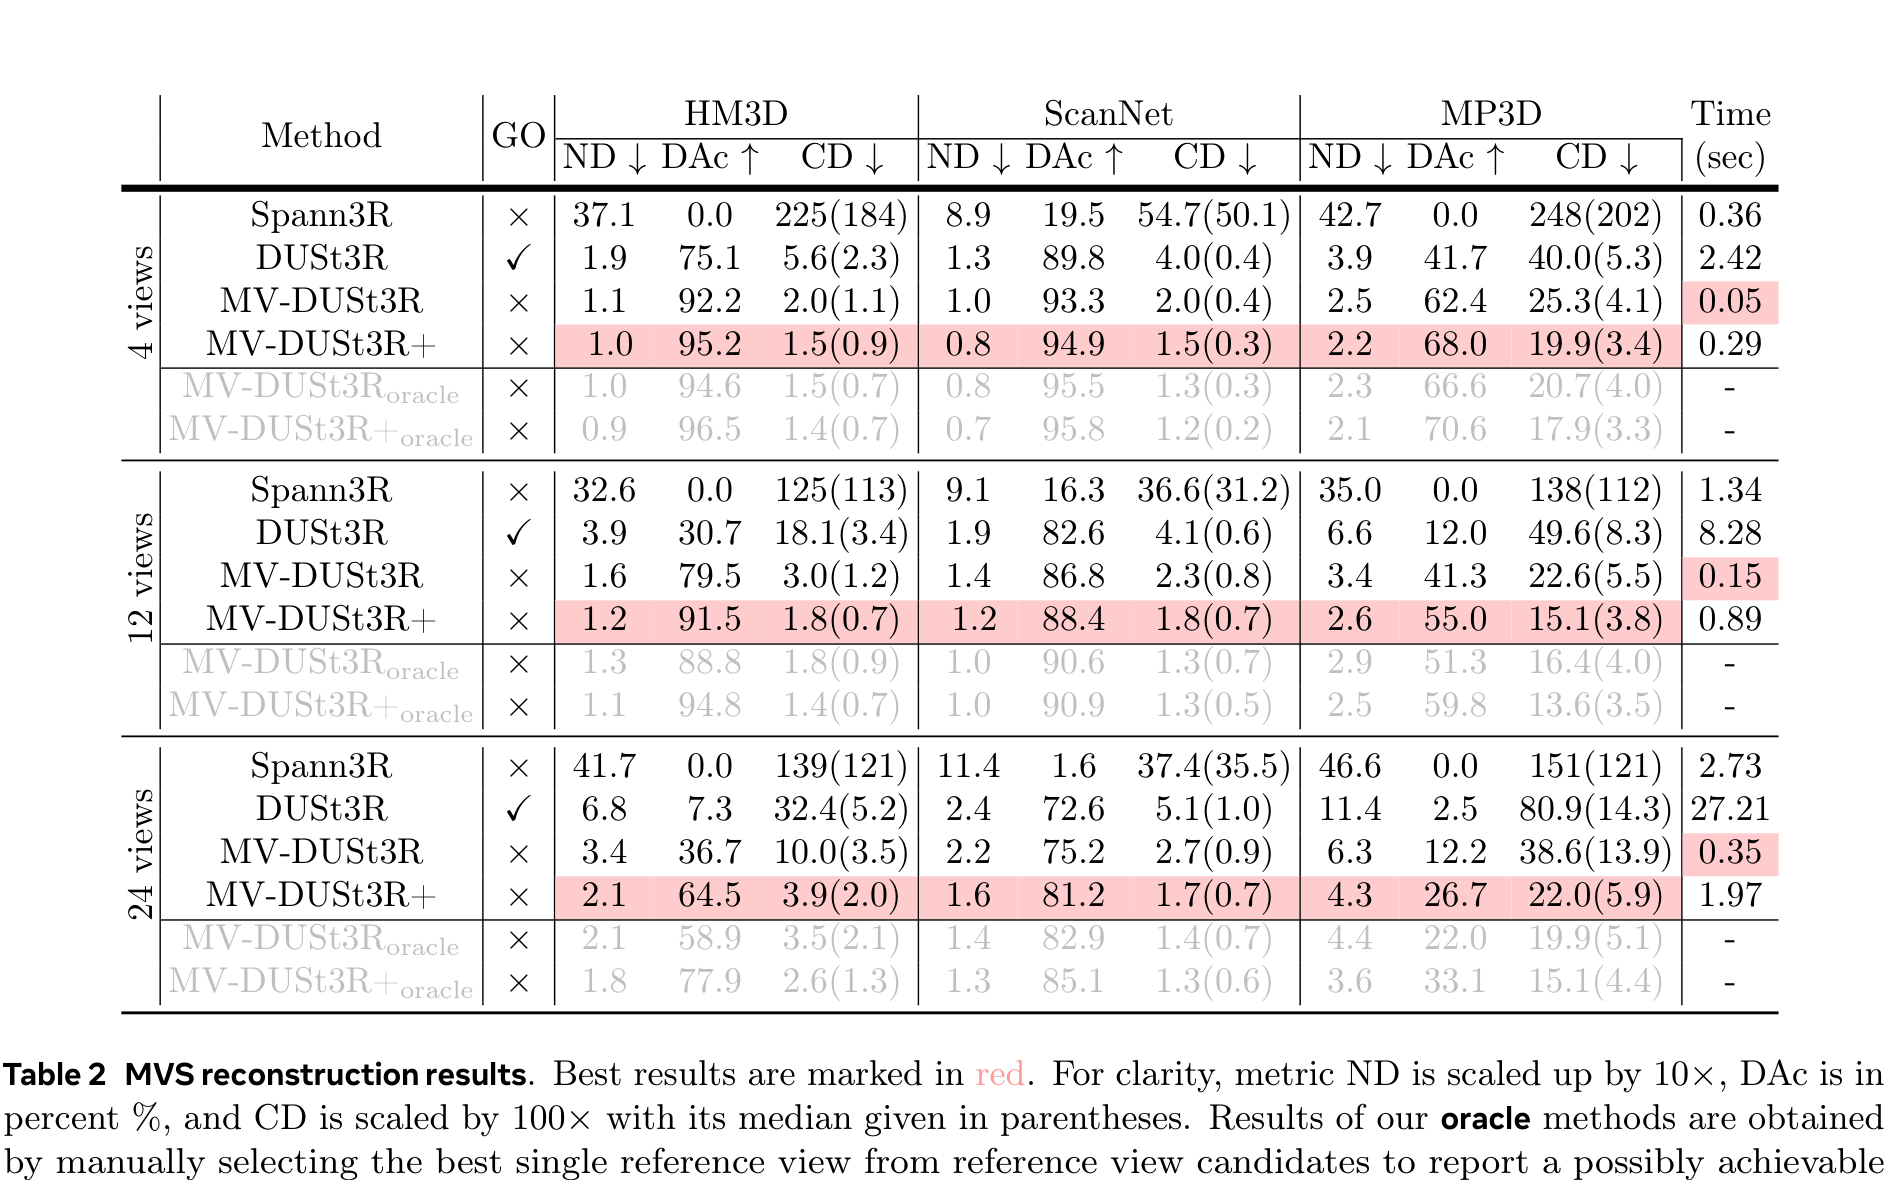
\includegraphics[height=0.62\textheight,keepaspectratio]{mvdust3r_results_table.png}

  \vspace{0.04cm}
  {\scriptsize Across multiple datasets and view counts, the highlighted rows show that MV-DUSt3R+ improves reconstruction quality while keeping runtime practical.}

  \figsource{Tang et al., MV-DUSt3R+, Table 2}
\end{frame}

\begin{frame}{Qualitative Motivation}
  \centering
  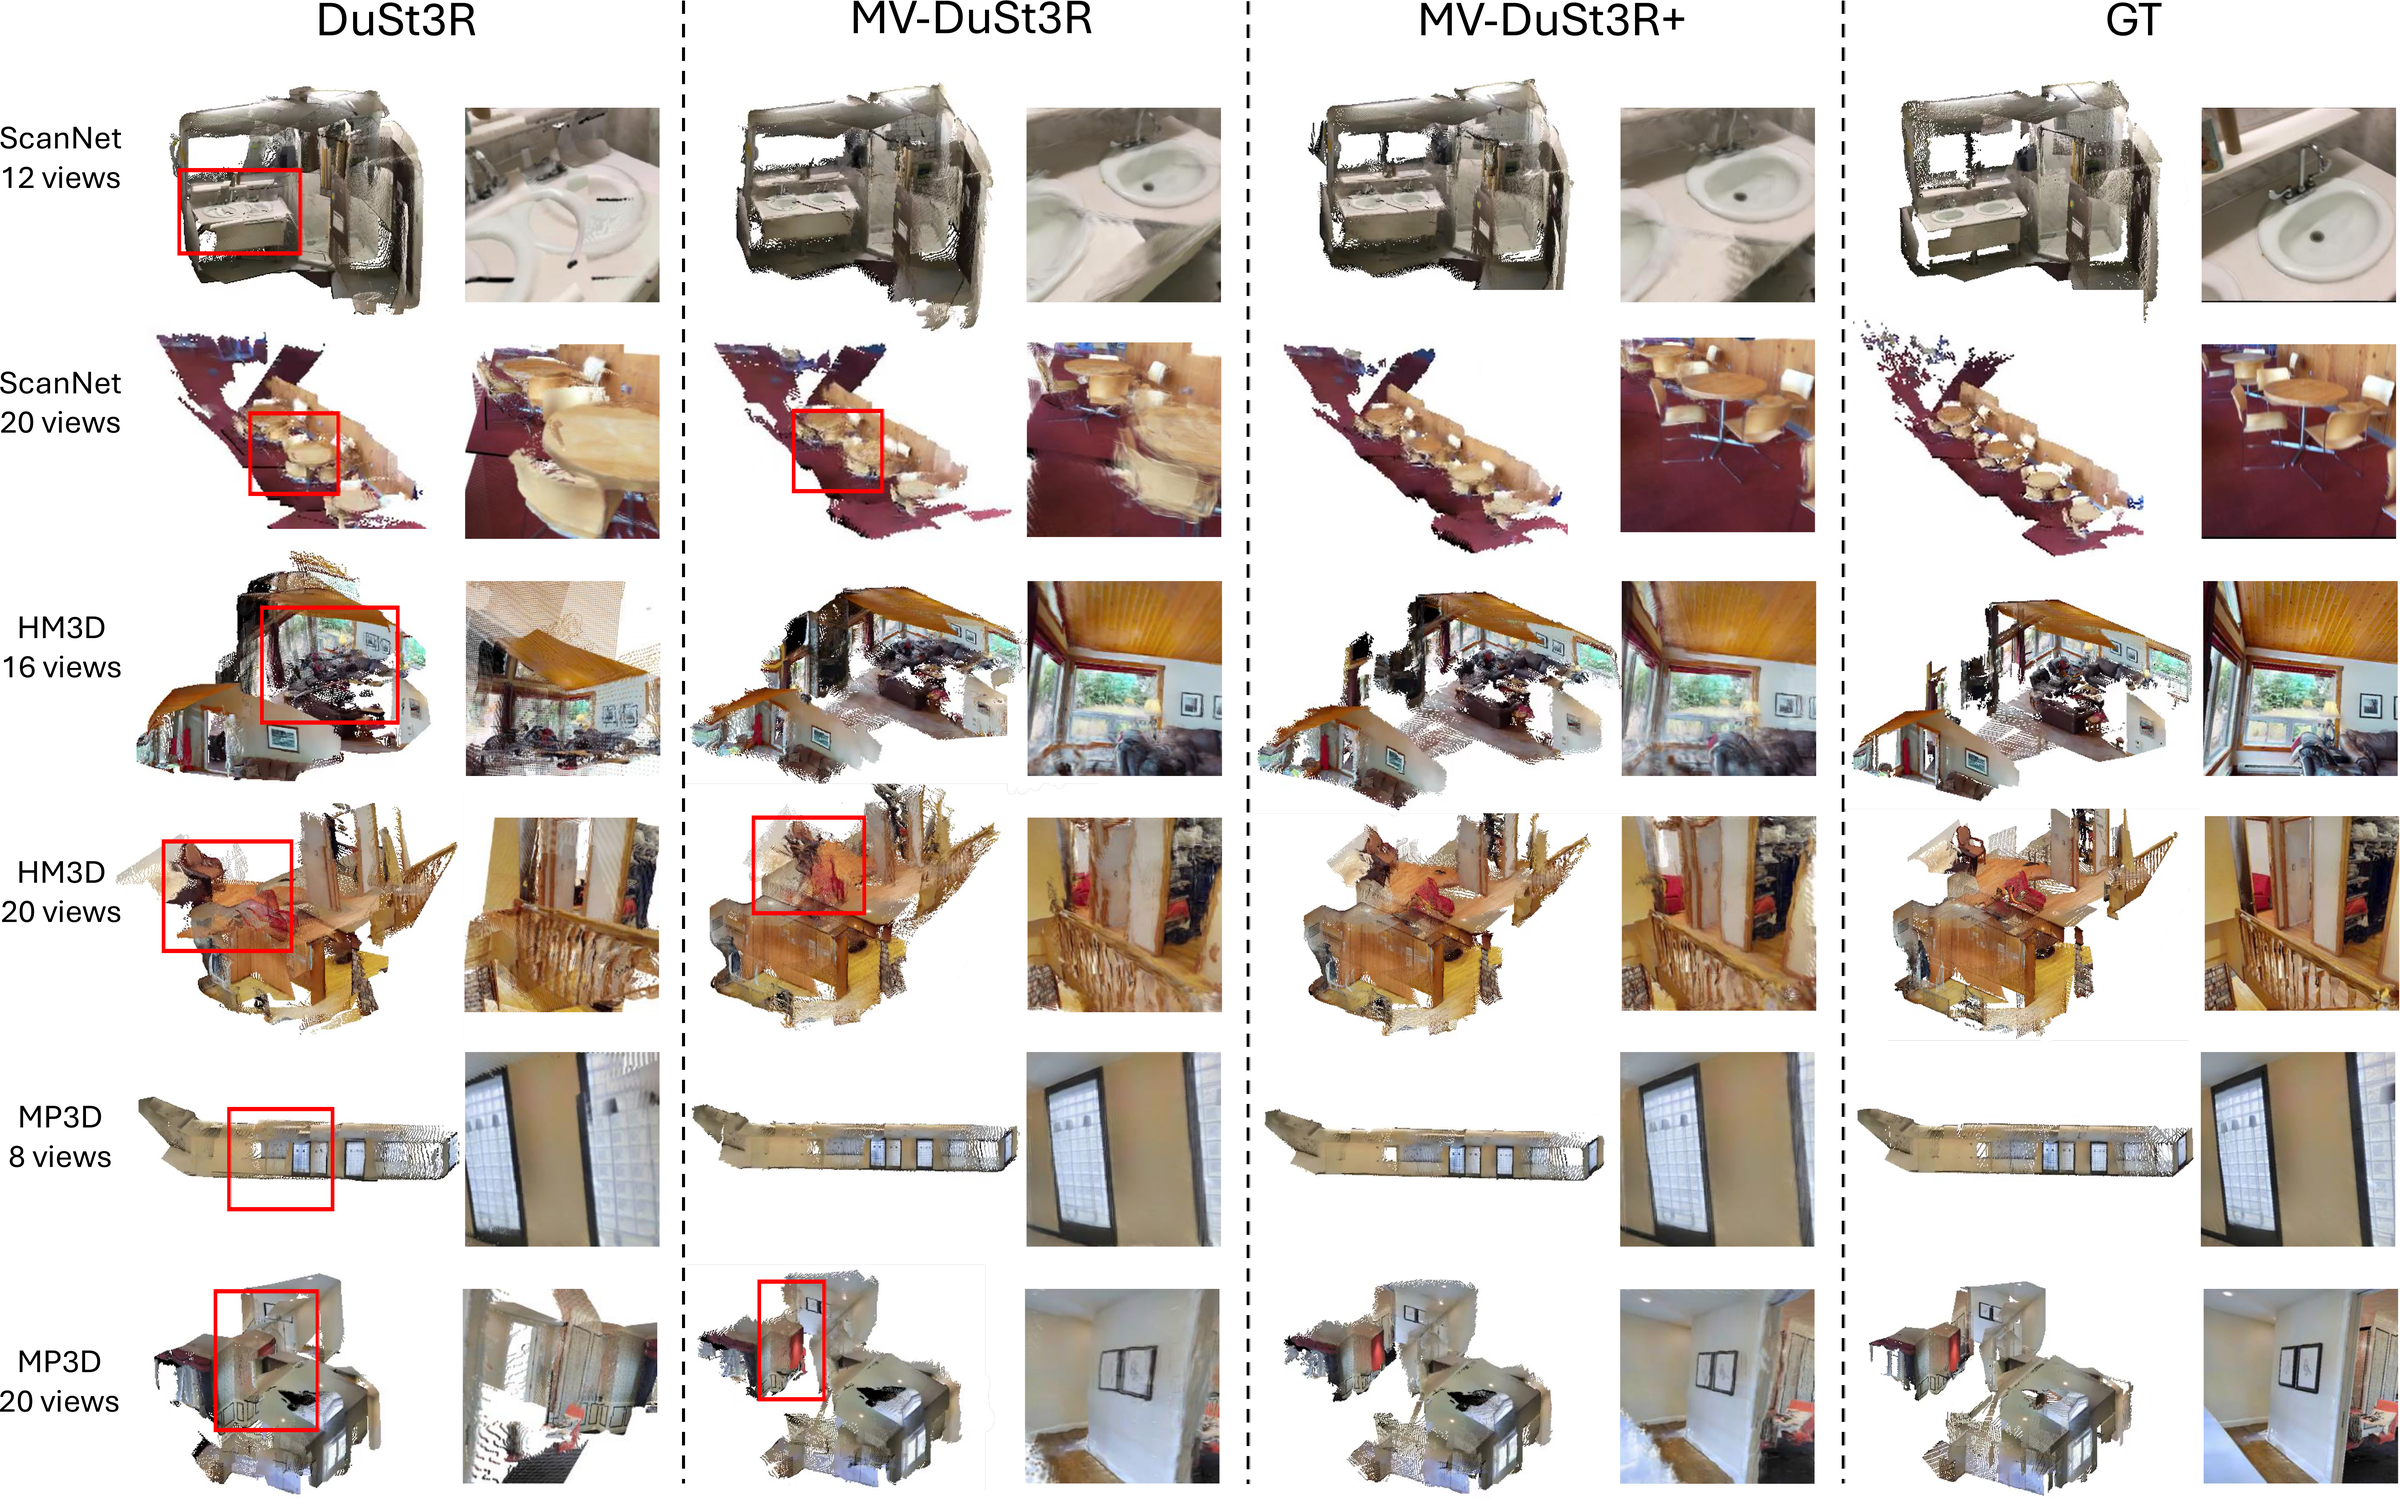
\includegraphics[height=0.65\textheight,keepaspectratio]{mv_qualitative_slide.png}

  \vspace{0.04cm}
  {\scriptsize DUSt3R often fails on repeated structures, while MV-DUSt3R+ remains more stable in sparse-view scenes.}

  \figsource{Tang et al., MV-DUSt3R+, qualitative results}
\end{frame}

\begin{frame}{Final Pipeline}
  \centering
  \begin{tikzpicture}[
    node distance=0.75cm,
    every node/.style={font=\small},
    box/.style={
      rectangle,
      rounded corners,
      draw=accent,
      fill=soft,
      align=center,
      minimum width=0.78\textwidth,
      minimum height=0.72cm
    },
    arr/.style={-{Latex[length=2.5mm]}, very thick, draw=accent}
  ]
    \node[box] (data) {Select sparse posed RGB-D views and scene-level train / validation / test splits};
    \node[box, below=of data] (subset) {Run MV-DUSt3R+ to produce candidate point cloud and confidence};
    \node[box, below=of subset] (base) {Use source depth maps with poses/intrinsics to anchor source rays};
    \node[box, below=of base] (heads) {Apply Run 30 selective source-depth correction};
    \node[box, below=of heads] (eval) {Evaluate overall, occlusion, and repeated/wrong-depth gates};

    \draw[arr] (data) -- (subset);
    \draw[arr] (subset) -- (base);
    \draw[arr] (base) -- (heads);
    \draw[arr] (heads) -- (eval);
  \end{tikzpicture}
\end{frame}

\begin{frame}{Experiment Variables}
  \begin{columns}[T]
    \column{0.48\textwidth}
    \textbf{Controlled factors}
    \begin{itemize}
      \item Number of input views
      \item RGB-D source depth availability
      \item Scene-level train / validation / test split
      \item Fixed Run 30 policy on final test
    \end{itemize}

    \column{0.48\textwidth}
    \textbf{Observed outcomes}
    \begin{itemize}
      \item Reconstruction accuracy
      \item Completeness and consistency
      \item Runtime per scene
      \item Occlusion and repeated/wrong-depth failures
    \end{itemize}
  \end{columns}
\end{frame}

\begin{frame}{RGB-only Diagnostic Path}
  \footnotesize
  \begin{enumerate}
    \item First build a supervised label cache with per-view visibility,
    occlusion, floating/wrong-depth, and match labels.
    \item Mine occlusion-heavy, low-overlap, and hard-negative subsets before
    training the learned heads.
    \item Freeze MV-DUSt3R+ and train small OARH / RSDH heads from generated
    labels, excluding direct target-label leakage features.
    \item Runs 22--26 move the heads into reconstruction-level validation gates
    with fixed-confidence, top-k, and all-candidate baselines.
    \item Run 27 is self-contained and learns a bounded confidence residual
    from actual candidates, self-geometry support, and raw image-patch cues.
    \item Completed Run 27 still selects all candidates: learned filtering beats
    fixed confidence but loses completeness against full retention.
    \item These runs motivate switching the final inference contract to RGB-D.
  \end{enumerate}
\end{frame}

\begin{frame}{RGB-D Source-Depth Correction}
  \footnotesize
  \begin{enumerate}
    \item Run 28 therefore preserves candidate count and learns source-ray
    3D corrections from training depth and poses, using no depth at inference.
    \item Completed Run 28 still fails the gate, but its source-depth oracle
    shows large occlusion and ambiguity headroom.
    \item Run 29 approximates that oracle with RGB-only monocular depth aligned
    through the input poses and intrinsics.
    \item Completed Run 29 regresses both occlusion and ambiguity, so RGB-only
    monodepth is not enough.
    \item Run 30 makes source depth an explicit RGB-D input and gates
    full/selective source-ray correction policies.
    \item Selected policy: \texttt{rgbd\_residual\_ge\_0.30}, residual mode,
    \(\alpha = 1.0\), threshold \(0.30m\).
    \item Final selected method: \texttt{rgbd\_source\_depth\_selected}.
    \item Keep final test clean: no threshold tuning, no checkpoint selection
    on test scenes.
  \end{enumerate}
\end{frame}

\begin{frame}{Datasets}
  \begin{columns}[T]
    \column{0.42\textwidth}
    \begin{block}{Primary dataset: ScanNet++}
      High-fidelity indoor scenes with registered DSLR images and commodity
      iPhone captures.
    \end{block}

    \begin{block}{Secondary dataset: DTU}
      Controlled object-centric scenes for supplementary evaluation and
      sanity checks in a cleaner setting.
    \end{block}

    \small If compute is limited, we will use curated subsets rather than the
    full datasets.

    \column{0.58\textwidth}
    \centering
    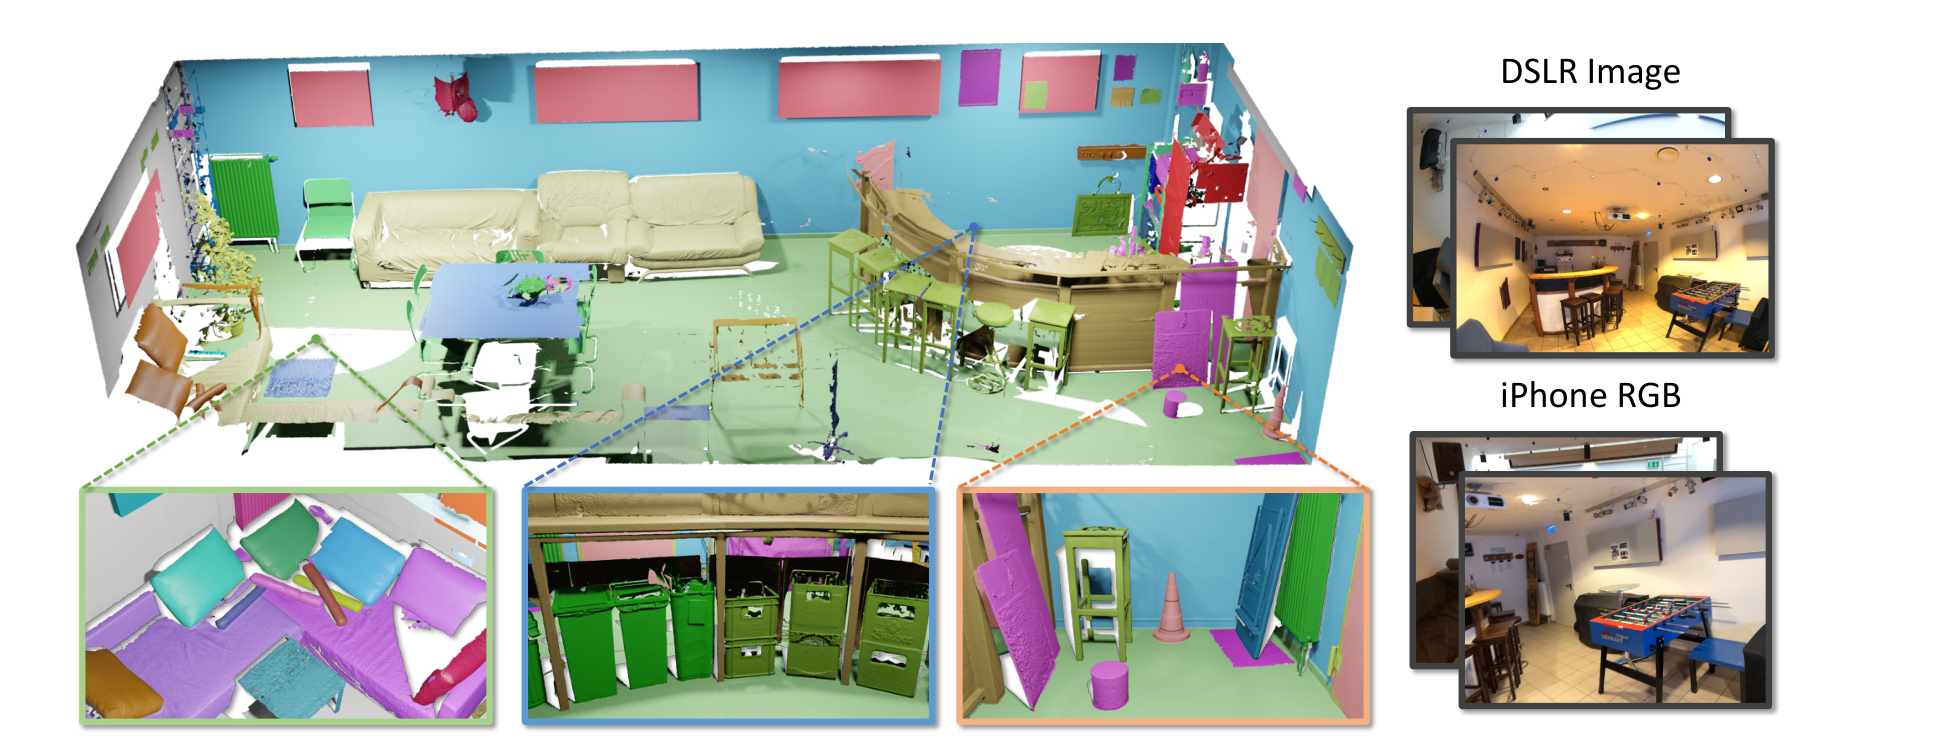
\includegraphics[width=\linewidth]{scannetpp_overview_crop.png}
  \end{columns}

  \vspace{0.08cm}
  \figsource{Yeshwanth et al., ScanNet++, ICCV 2023, Figure 1}
\end{frame}

\begin{frame}{Why ScanNet++?}
  \begin{columns}[T]
    \column{0.63\textwidth}
    \centering
    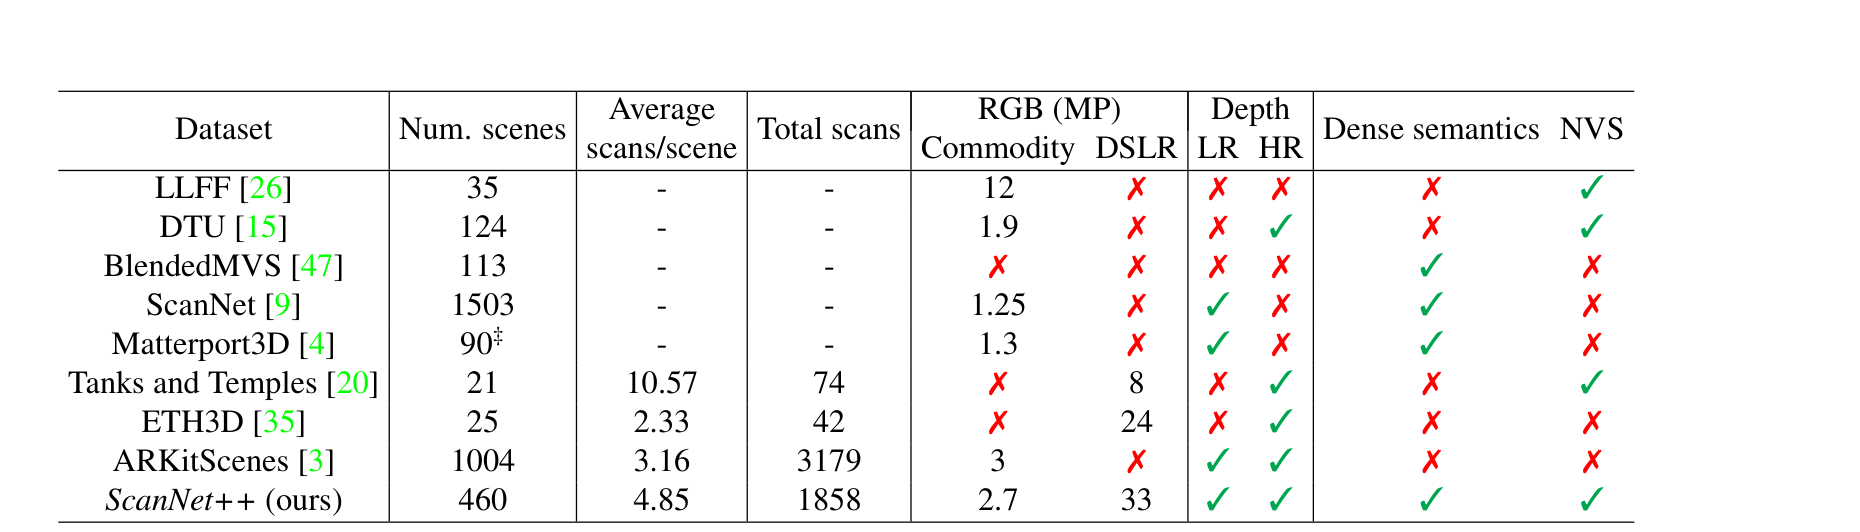
\includegraphics[width=\linewidth]{scannetpp_table_crop.png}

    \column{0.37\textwidth}
    \begin{itemize}
      \item 460 indoor scenes with high-fidelity geometry
      \item DSLR images support stronger geometric supervision
      \item Commodity captures make sparse-view testing realistic
      \item Dense semantics and NVS setup make the benchmark richer
    \end{itemize}
  \end{columns}

  \vspace{0.08cm}
  \figsource{Yeshwanth et al., ScanNet++, ICCV 2023, Table 1}
\end{frame}

\begin{frame}{Evaluation Plan}
  \small
  \begin{columns}[T]
    \column{0.52\textwidth}
    \begin{itemize}
      \item Reconstruction F-score against available ground-truth geometry
      \item Accuracy, completeness, and Chamfer distance of point clouds
      \item Sparse 2--5 view behavior across scene splits
      \item Limit-specific gates for occlusion and wrong-depth ambiguity
      \item Runtime per scene for practical inference
    \end{itemize}

    \vspace{0.08cm}
    \begin{block}{Success criterion}
      Run 30 must beat the best non-learned baseline overall and improve both
      occlusion and ambiguity subsets by at least the gate margin.
    \end{block}

    \column{0.48\textwidth}
    \centering
    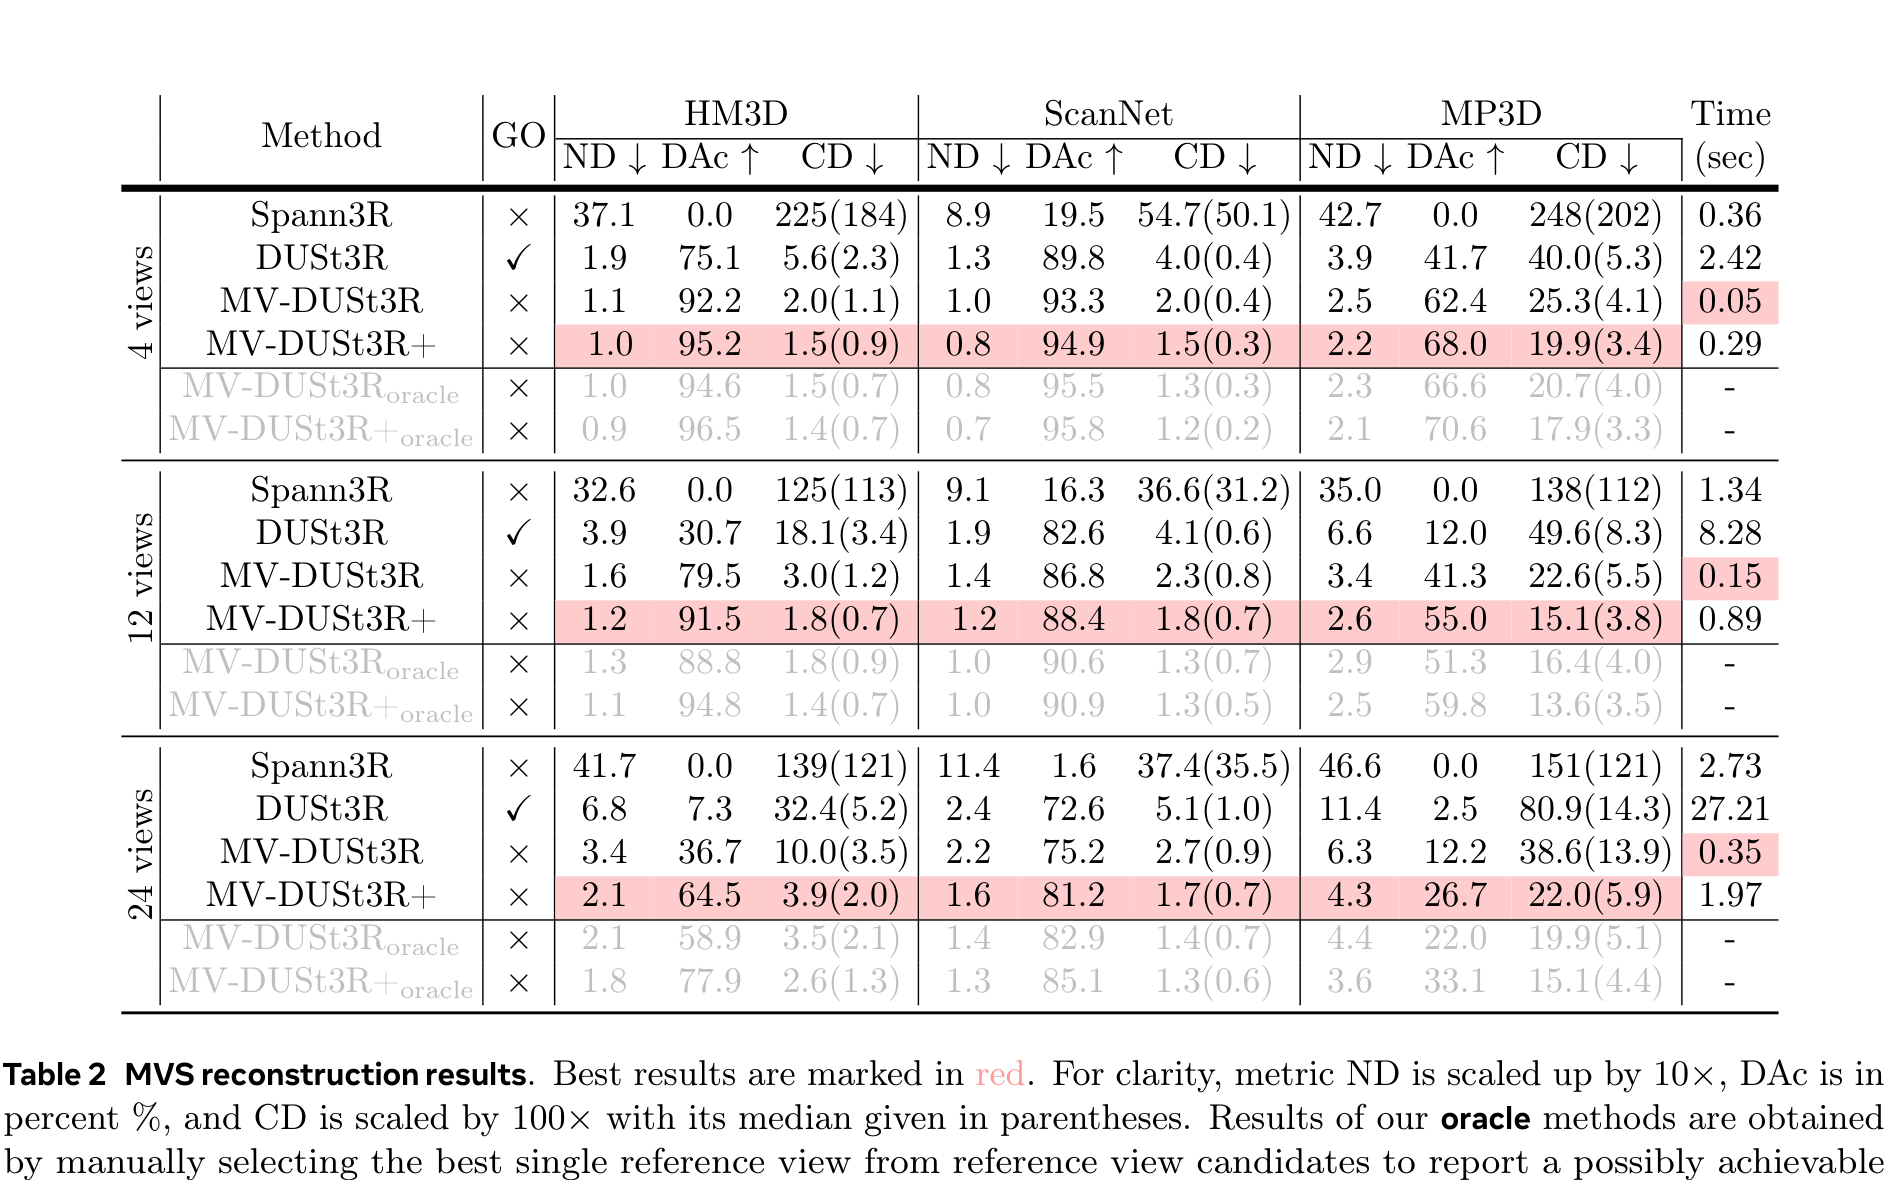
\includegraphics[height=0.46\textheight,keepaspectratio]{mvdust3r_results_table.png}

    \vspace{0.04cm}
    \figsource{Tang et al., MV-DUSt3R+, quantitative benchmark}
  \end{columns}
\end{frame}

\begin{frame}{Final RGB-D Result}
  \scriptsize
  \begin{block}{Run 30 gate decision}
    \texttt{selected\_method = rgbd\_source\_depth\_selected};
    best baseline = \texttt{all\_candidates};
    gate margin = 0.005;
    \texttt{pass\_all\_limits = 1}.
  \end{block}

  \vspace{0.08cm}
  \centering
  \begin{tabular}{lrrrr}
    \toprule
    \textbf{Split/subset} & \textbf{All cand.} & \textbf{Fixed conf.} &
    \textbf{RGB-D selected} & \textbf{Delta vs all} \\
    \midrule
    Val overall & 0.1194 & 0.1123 & 0.1753 & +0.0559 \\
    Val occlusion & 0.1064 & 0.0917 & 0.2522 & +0.1458 \\
    Val ambiguity & 0.1623 & 0.1416 & 0.3000 & +0.1377 \\
    \midrule
    Test overall & 0.1758 & 0.1662 & 0.2764 & +0.1007 \\
    Test occlusion & 0.2111 & 0.1866 & 0.3146 & +0.1035 \\
    Test ambiguity & 0.1621 & 0.1462 & 0.2948 & +0.1327 \\
    \bottomrule
  \end{tabular}
\end{frame}

\begin{frame}{Why RGB-D Works}
  \footnotesize
  \begin{alertblock}{Final wording}
    RGB-only learned extensions did not pass reconstruction-level gates. After
    switching the inference contract to RGB-D, Run 30 uses input source depth
    maps with known camera poses/intrinsics for source-ray correction and passes
    the overall, occlusion, and ambiguity gates on held-out scenes.
  \end{alertblock}

  \begin{itemize}
    \item Source depth anchors each source ray to metric geometry.
    \item Correction preserves candidate count, unlike filtering that hurts
    recall and completeness.
    \item Occlusion and repeated/wrong-depth cases improve because the method
    fixes geometry rather than discarding sparse-view evidence.
  \end{itemize}
\end{frame}

\begin{frame}{Expected Deliverables}
  \begin{itemize}
    \item End-to-end implementation for training and evaluation
    \item Quantitative results on unseen scenes across multiple view counts
    \item Qualitative 3D visualizations and failure-case analysis
    \item Final report discussing strengths, limitations, and recommendations
    \item Reproducible Kaggle experiment scripts organized under
    \texttt{scripts/kaggle}
    \item Submitted supervised-extension kernels for Run 12 and Run 13
    \item Clean GitHub repository with curated docs, proposal sources, and PDF
    deck
  \end{itemize}
\end{frame}

\begin{frame}{Expected Contributions}
  \begin{itemize}
    \item A focused benchmark of sparse-view reconstruction on unseen scenes
    \item A direct comparison between pairwise and single-stage multi-view
    reasoning
    \item Evidence about when sparse-view reconstruction remains reliable
    \item Practical guidance for follow-up work on robust 3D reconstruction
    \item An ablation record showing which proposed modules help and which fail
    \item A supervised follow-up plan for occlusion reliability and
    repeated-structure match disambiguation
  \end{itemize}
\end{frame}

\begin{frame}{References}
  \footnotesize
  \begin{itemize}
    \item Wang et al., ``DUSt3R: Geometric 3D Vision Made Easy,'' CVPR 2024.
    \item Tang et al., ``MV-DUSt3R+: Single-Stage Scene Reconstruction from
    Sparse Views In 2 Seconds,'' CVPR 2025.
    \item Yeshwanth et al., ``ScanNet++: A High-Fidelity Dataset of 3D Indoor
    Scenes,'' ICCV 2023.
    \item DTU Robot Image Data Sets, Multi-View Stereo Benchmark.
  \end{itemize}
\end{frame}


\end{document}
